\clearpage{\pagestyle{empty}\cleardoublepage}
\chapter*{Introduzione} 
%%\markboth{Introduzione}{Introduzione}
\addcontentsline{toc}{chapter}{Introduzione}
%

%
Il rapporto sullo stato del solare fotovoltaico in 
Italia\cite{gse2010} pubblicato dal \emph{Gestore dei Servizi Energetici}
(GSE) nell'Aprile del 2011, mostra come, negli ultimi anni, 
l'utilizzo di tale tecnologia ai fini della produzione di energia
elettrica da immettere in rete abbia vissuto una crescita 
decisamente sostenuta.
%
Solo nel 2010, infatti, il numero di impianti fotovoltaici presenti
sul territorio nazionale \`e aumentato di 84.689 unit\`a, andando
a raddoppiare il numero di impianti esistenti a fine 2009.
%
Nello stesso anno, la potenza \`e addirittura triplicata: 
sono stati installati complessivamente 2.326 MW.
%

%
\begin{figure}[!h]
\centering
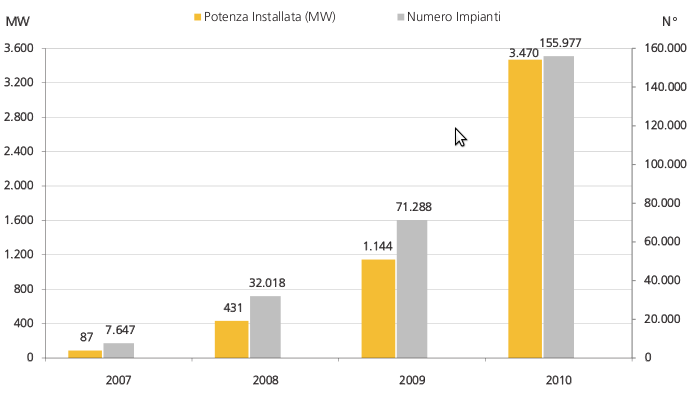
\includegraphics[width=350pt]{img/trend-fotovoltaico-italia.png}
\caption{Trend di crescita del fotovoltaico in Italia}
\label{fotovoltaico-italia}
\end{figure}
%

%
I dati del 2010 si inseriscono all'interno di un trend di crescita 
iniziato, ormai, pi\`u di tre anni fa, come \`e possibile verificare
osservando l'istogramma in figura \ref{fotovoltaico-italia}.
%

%
Le ragioni di questo trend di crescita, definito \emph{straordinario} in 
\cite{gse2010}, sono in parte attribuibili ai recenti sviluppi della
tecnologia fotovoltaica, che hanno portato alla realizzazione di moduli
sempre pi\`u efficienti e sempre meno costosi.
%
D'altro canto, una enorme spinta \`e arrivata dal programma di
incentivazione\footnote{comunemente noto come \emph{Conto Energia}.} previsto dalla direttiva europea 2001/77/CE, recepita in 
Italia mediante approvazione ed emanazione del decreto legislativo 387 
del 2003\cite{camera2003}.
%% ma ci sono anche gli incentivi, 
%% ==> molti piccoli impianti
%% ==> necessita` di sistemi di monitoraggio

%% descrizione del contenuto della tesi
